\chapter{Escalamiento}

Scrum es aconsejable para ser óptimo en equipos chicos y proyectos pequeños, con agrupación de personas de múltiples disciplinas en un solo equipo para maximizar el ancho de banda de las comunicaciones, la visibilidad y la confianza. Esto sucede porque cuando los equipos son grandes aumenta el acoplamiento de individuos complejizando las comunicaciones y dificultando la coordinación y el buen desarrollo de las reuniones Scrum. Además se desprende del principio o Ley de Brooks, que dice que cuando se agregan personas a un proyecto o equipo aumentan los canales de comunicación pudiendo generar sobrecarga de comunicación. Por este motivo y desde un punto de vista purista, cuando se quiere implementar Scrum en proyectos grandes que requieren muchas personas, en su forma ortodoxa, no es recomendable. Pero se han encontrado maneras organizativas para aplicar Scrum en estos casos. Una forma es el uso de equipos Scrum de características, equipos Scrum de componentes y algún sistema de integración como el uso de "Scrum de Scrum" y de Equipos de Product Owners.

\section{Equipos de características}

Abordar el problema de proyectos grandes con "Equipos Scrum de características" consiste en la conformación de equipos totalmente multi-funcionales con un enfoque "Whole Team"\footnote{En un enfoque Whole Team todos pueden hacer, hasta cierta medida, alguna tarea de otro\cite{Juan-Gabardini-2015}.}, capaces de operar en todos los niveles de la arquitectura del producto con el fin de ofrecer las características centradas en el cliente (ver figura \ref{fig:ScrumTeamsByFeatures}). O sea que cada equipos trabaja sobre determinadas características de producto (Features) o PBIs desarrollando todos los niveles del sistema a desarrollar (end-to-end). En este sentidos, los equipos son homogéneos entre sí pero heterogéneos internamente, con integrantes de habilidades diversas y características profesionales multidisciplinares. Para lograr esto se debe conformar una organización de aprendizaje donde los equipos practican el aprendizaje continuo, donde aprenden para abarcar los componentes arquitectónicos.

\begin{figure}[h]
  \centering
  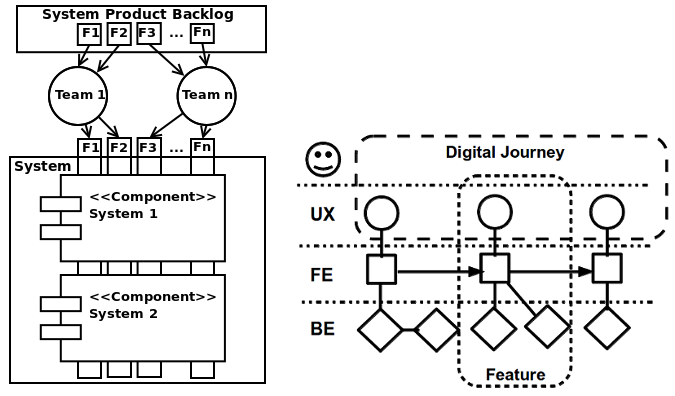
\includegraphics[width=0.80\textwidth]{ScrumTeamsByFeatures}
  \caption{Esquema de Equipos de Características}
  \centering
  \label{fig:ScrumTeamsByFeatures} %\ref{fig:ScrumTeamsByFeatures}
\end{figure}

En esta arquitectura de organización es necesario coordinar el trabajo de los diferentes equipos. Los Scrum Master deben reunirse con regularidad, promoviendo la transformación a través de una lista visible de los impedimentos de organización. Los Scrum Master, además deberán estar familiarizados con biografía relacionada a este problema de escalabilidad como "Scaling Lean and Agile Development" \cite{Larman-Vodde-2008}.

\section{Equipos de componentes}

Abordar el problema de proyectos grandes con "Equipos Scrum de componentes" (ver figura \ref{fig:ScrumTeamsByComponent}) consiste en que cada equipo sólo es responsable de la ejecución de ciertos componentes dedicados en el sistema de los cuales el equipo es dueño de su desarrollo. Desde esta perspectiva se pueden tener equipos dedicados por capas (capa front-end, capa de servicios, capa de persistencia) y por componentes de arquitectura de software (diferentes componentes como librerías, servicios o subsistemas).

\begin{figure}[h]
  \centering
  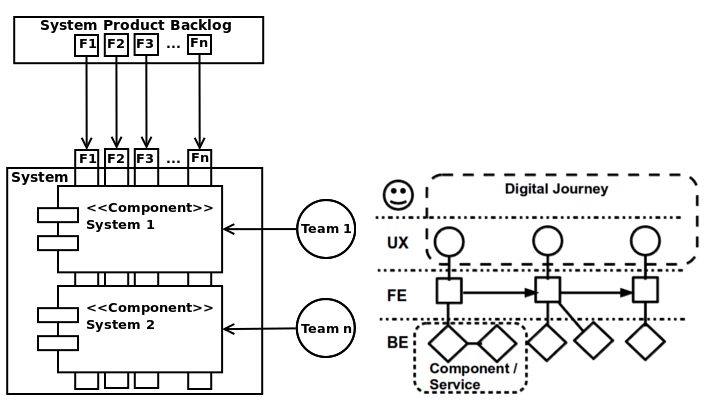
\includegraphics[width=0.80\textwidth]{ScrumTeamsByComponent}
  \caption{Esquema de Equipos de Características}
  \centering
  \label{fig:ScrumTeamsByComponent} %\ref{fig:ScrumTeamsByComponent}
\end{figure}

Para terminar una PBI o historia de usuario hay en la mayoría de los casos la necesidad de dividir las historias en partes más pequeñas que podrían ser implementadas dentro de un solo componente. Además se genera dependencias entre los diferentes equipos haciendo necesario procesos de integración periódica y coordinación de equipos. En muchos casos, una sola historia de usuario no se puede implementar dentro de un único sprint y, en su defecto, depende de los resultados de otras historias desarrolladas por otro equipo que aún no están disponibles. A esto se lo llama "pipeline" y debe evitarse en lo posible o gestionarse apropiadamente.

La ventaja de utilizar equipos de componentes es que es más fácil asegurar una determinada arquitectura del sistema. Por ejemplo si se quiere asegurar una Arquitectura SOA o una de Microservicios que está orientada a componentes. Esta idea está, entre otras cosas, basada en la "Ley de Conway"\footnote{Conway's Law \cite{Conway-1968} no es exactamente una ley, sino que es más bien una observación que Conway publicó en 1968.} que sugiere que las organizaciones pueden replicar su arquitectura en los productos que ellas producen \cite{Martin-Fowler-2014}. 

Por otro lado, puede tener como desventaja que las personas se pueden especializar sólo en pequeñas partes del sistema y el conocimiento global sobre el sistema en su conjunto podría perderse \cite{Scrum-Institute-2015}. En este caso podría tener lugar una optimización local, ya que el equipo a veces puede tomar decisiones que están optimizadas para el componente individual, pero las mejores soluciones desde una perspectiva del sistema total podrían haber sido desestimadas u obviadas.


\section{Equipos mixtos}

También es posible la configuración de equipos mixtos que son la combinación de equipos de características y de componentes (ver figura \ref{fig:ScrumTeamsMix}).

\begin{figure}[h]
  \centering
  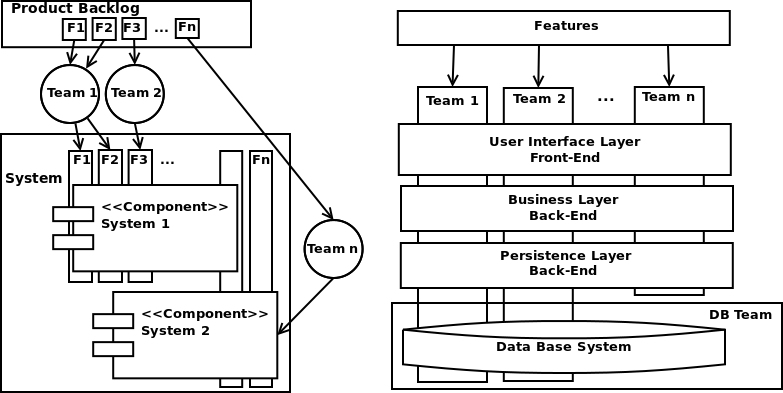
\includegraphics[width=0.99\textwidth]{ScrumTeamsMix}
  \caption{Ejemplo de equipos mixtos.}
  \centering
  \label{fig:ScrumTeamsMix} %\ref{fig:ScrumTeamsMix}
\end{figure}

\section{Scrum de Scrum}

Scrum de Scrum es una forma de organización y técnica para escalar Scrum a grupos grandes de personas u organizaciones con proyectos grandes, programas o portfolios. Consiste en distinguir un integrante con el rol de Embajador, denominado "Ambassador", por cada Equipo Scrum \cite{Stefanini-2013}. El Embajador será quien participará en reuniones Daily con Embajadores de otros equipos. A esta reunión de Embajadores se la llama "Scrum de Scrum" o SoS. Habitualmente se usa que el rol de Embajador lo desempeñe el Scrum Master, pero puede ser desempeñado por otro integrante del Equipo de Desarrollo. También puede ser desempeñado por un integrante del Equipo acompañado del Scrum Master.

La reunión SoS se comporta como una Daily donde los Embajadores reportan la situación de su equipo y sus impedimentos. El embajador de cada equipo comenta la respuesta a las siguientes tres preguntas:

\begin{itemize}
\item \textbf{¿Qué hicimos ayer?}
\item \textbf{¿Qué vamos a hacer hoy?}
\item \textbf{Si tenemos obstáculos: ¿Qué impedimentos tenemos?} ¿Qué impedimentos tenemos a nivel de equipo? ¿Si algún otro equipo nos bloquea para algo? ¿Si bloqueamos en algo a algún otro equipo?
\end{itemize}

La SoS puede ser facilitada y moderada por una persona que puede desempeñar un rol de facilitador, coordinador e integrador inter-equipos. Este rol puede tener diferentes nombres y el SBOK lo denomina Chief Scrum Master o CSM. El CSM apoyará y brindará soporte a los SM de diferentes equipos.

\subsection{Scrum of Scrum de Scrums}

En organizaciones donde hay muchos Equipo Scrums trabajando en varias partes de un proyecto o producto grande puede ser necesaria otro nivel más de coordinación, ya que hay equipos que no participan en SoS de otras áreas. Aquí es cuando se aplica la "Scrum of Scrum de Scrums"\footnote{\cite{SBOK-2013}} o SoSoS, que consiste en una reunión frecuente a un nivel superior de la SoS.
